\subsection{Vignet  Class Reference}
\label{class_vignet}\index{Vignet@{Vignet}}
Similar to {\bf Kernel} {\rm (p.\,\pageref{class_kernel})}, but resizeable and contains some kind of {\bf Point} {\rm (p.\,\pageref{class_point})}. 


{\tt \#include $<$vignet.h$>$}

Inheritance diagram for Vignet::\begin{figure}[H]
\begin{center}
\leavevmode
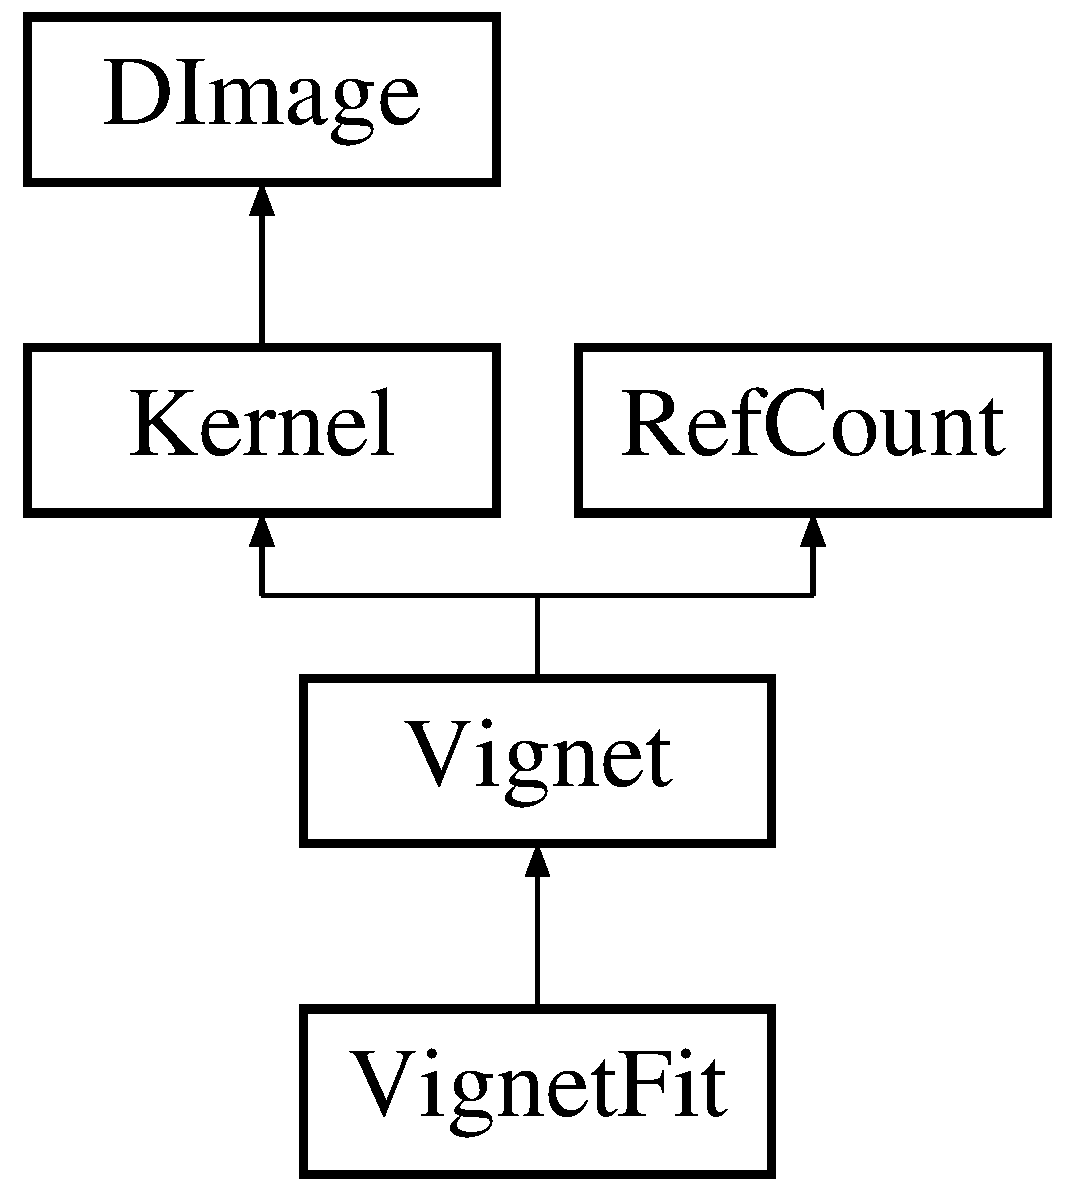
\includegraphics[height=4cm]{class_vignet}
\end{center}
\end{figure}
\subsubsection*{Public Methods}
\begin{CompactItemize}
\item 
\index{Vignet@{Vignet}!Vignet@{Vignet}}\index{Vignet@{Vignet}!Vignet@{Vignet}}
{\bf Vignet} (const double \&X, const double \&Y, const {\bf Image} \&Source, const int HMax\-X, const int HMax\-Y)\label{class_vignet_a0}

\item 
\index{Vignet@{Vignet}!Vignet@{Vignet}}\index{Vignet@{Vignet}!Vignet@{Vignet}}
{\bf Vignet} (const double \&X, const double \&Y, const int HMax\-X, const int HMax\-Y)\label{class_vignet_a1}

\item 
\index{Vignet@{Vignet}!Vignet@{Vignet}}\index{Vignet@{Vignet}!Vignet@{Vignet}}
{\bf Vignet} (const string \&File\-Name)\label{class_vignet_a2}

\item 
\index{Vignet@{Vignet}!Vignet@{Vignet}}\index{Vignet@{Vignet}!Vignet@{Vignet}}
{\bf Vignet} ()\label{class_vignet_a3}

\item 
\index{~Vignet@{$\sim$Vignet}!Vignet@{Vignet}}\index{Vignet@{Vignet}!~Vignet@{$\sim$Vignet}}
{\bf $\sim$Vignet} ()\label{class_vignet_a4}

\item 
\index{Resize@{Resize}!Vignet@{Vignet}}\index{Vignet@{Vignet}!Resize@{Resize}}
void {\bf Resize} (const int HSize\-X, const int HSize\-Y)\label{class_vignet_a5}

\item 
\index{Resize@{Resize}!Vignet@{Vignet}}\index{Vignet@{Vignet}!Resize@{Resize}}
void {\bf Resize} (const double \&Scale\-Factor)\label{class_vignet_a6}

\item 
\index{Detect@{Detect}!Vignet@{Vignet}}\index{Vignet@{Vignet}!Detect@{Detect}}
void {\bf Detect} (const double \&Pos\-Thresh, const double \&Neg\-Thresh)\label{class_vignet_a7}

\item 
\index{Aperture@{Aperture}!Vignet@{Vignet}}\index{Vignet@{Vignet}!Aperture@{Aperture}}
double {\bf Aperture} (double \&Var\-Aper, const double \&Radius, const double \&Var\-Pix, const double \&Sky) const\label{class_vignet_a8}

\item 
\index{WeightedAperture@{WeightedAperture}!Vignet@{Vignet}}\index{Vignet@{Vignet}!WeightedAperture@{Weighted\-Aperture}}
double {\bf Weighted\-Aperture} (double \&Var\-Aper, const {\bf Kernel} \&Model, const double \&Var\-Pix, const double \&Sky) const\label{class_vignet_a9}

\item 
\index{WeightedRecentroid@{WeightedRecentroid}!Vignet@{Vignet}}\index{Vignet@{Vignet}!WeightedRecentroid@{Weighted\-Recentroid}}
void {\bf Weighted\-Recentroid} (double \&Flux, const double \&Sky, const double \&Sig\-X, const double \&Sigy)\label{class_vignet_a10}

\item 
\index{Hx@{Hx}!Vignet@{Vignet}}\index{Vignet@{Vignet}!Hx@{Hx}}
int {\bf Hx} () const\label{class_vignet_a11}

\item 
\index{Hy@{Hy}!Vignet@{Vignet}}\index{Vignet@{Vignet}!Hy@{Hy}}
int {\bf Hy} () const\label{class_vignet_a12}

\item 
\index{readFits@{readFits}!Vignet@{Vignet}}\index{Vignet@{Vignet}!readFits@{read\-Fits}}
void {\bf read\-Fits} (const string \&File\-Name)\label{class_vignet_a13}

\begin{CompactList}\small\item\em write and read the {\bf DImage} {\rm (p.\,\pageref{class_dimage})} as a FITS array.\item\end{CompactList}\item 
\index{writeFits@{writeFits}!Vignet@{Vignet}}\index{Vignet@{Vignet}!writeFits@{write\-Fits}}
void {\bf write\-Fits} (const string \&File\-Name) const\label{class_vignet_a14}

\end{CompactItemize}
\subsubsection*{Public Attributes}
\begin{CompactItemize}
\item 
\index{ic@{ic}!Vignet@{Vignet}}\index{Vignet@{Vignet}!ic@{ic}}
int {\bf ic}\label{class_vignet_m0}

\begin{CompactList}\small\item\em coordinates of the center pixel where the Vignet was grabbed from.\item\end{CompactList}\item 
\index{jc@{jc}!Vignet@{Vignet}}\index{Vignet@{Vignet}!jc@{jc}}
int {\bf jc}\label{class_vignet_m1}

\begin{CompactList}\small\item\em coordinates of the center pixel where the Vignet was grabbed from.\item\end{CompactList}\item 
\index{dxc@{dxc}!Vignet@{Vignet}}\index{Vignet@{Vignet}!dxc@{dxc}}
double {\bf dxc}\label{class_vignet_m2}

\begin{CompactList}\small\item\em real coordinates of the star centroid relative to the down-left corner of center pixel (ic,jc).\item\end{CompactList}\item 
\index{dyc@{dyc}!Vignet@{Vignet}}\index{Vignet@{Vignet}!dyc@{dyc}}
double {\bf dyc}\label{class_vignet_m3}

\begin{CompactList}\small\item\em real coordinates of the star centroid relative to the down-left corner of center pixel (ic,jc).\item\end{CompactList}\item 
\index{istart@{istart}!Vignet@{Vignet}}\index{Vignet@{Vignet}!istart@{istart}}
int {\bf istart}\label{class_vignet_m4}

\begin{CompactList}\small\item\em image coordinates of the down-left corner pixel where the Vignet was grabbed.\item\end{CompactList}\item 
\index{jstart@{jstart}!Vignet@{Vignet}}\index{Vignet@{Vignet}!jstart@{jstart}}
int {\bf jstart}\label{class_vignet_m5}

\begin{CompactList}\small\item\em image coordinates of the down-left corner pixel where the Vignet was grabbed.\item\end{CompactList}\item 
\index{iend@{iend}!Vignet@{Vignet}}\index{Vignet@{Vignet}!iend@{iend}}
int {\bf iend}\label{class_vignet_m6}

\begin{CompactList}\small\item\em image coordinates of the upper-right corner pixel where the Vignet was grabbed.\item\end{CompactList}\item 
\index{jend@{jend}!Vignet@{Vignet}}\index{Vignet@{Vignet}!jend@{jend}}
int {\bf jend}\label{class_vignet_m7}

\begin{CompactList}\small\item\em image coordinates of the upper-right corner pixel where the Vignet was grabbed.\item\end{CompactList}\end{CompactItemize}
\subsubsection*{Protected Attributes}
\begin{CompactItemize}
\item 
\index{hx@{hx}!Vignet@{Vignet}}\index{Vignet@{Vignet}!hx@{hx}}
int {\bf hx}\label{class_vignet_n0}

\item 
\index{hy@{hy}!Vignet@{Vignet}}\index{Vignet@{Vignet}!hy@{hy}}
int {\bf hy}\label{class_vignet_n1}

\end{CompactItemize}


\subsubsection{Detailed Description}
Similar to {\bf Kernel} {\rm (p.\,\pageref{class_kernel})}, but resizeable and contains some kind of {\bf Point} {\rm (p.\,\pageref{class_point})}.



The documentation for this class was generated from the following file:\begin{CompactItemize}
\item 
{\bf vignet.h}\end{CompactItemize}
